\chapter{\difficult{Higher-dimensional Geometry}}\label{chapter:hdg}

    In this chapter, certain constructions and theorems introduced in the previous chapters are generalized to the setting of supergeometries and higher categories. As such, it can been as an analogue to \cref{chapter:hda} for (differential) geometry.

    The main references are~\citet{schreiber_loop_2005,baez_higher_2005}. The section on spectral geometry is based on~\citet{sanders_commutative_2012}, whereas that on smooth spaces is inspired by~\citet{baez_convenient_2011}. For an introduction to (higher) category theory, see \cref{chapter:cat}. \Cref{section:higher_lie_structures} gives a different approach to the higher-dimensional analogues of Lie algebras. For an introduction to supergeometry, see~\citet{cattaneo_introduction_2011}.

    \todo{CITE MORE (e.g. BARTELS, ...)}

    \minitoc

\section{Graded manifolds}

    In this section, some of the notions from \cref{part:diffgeom} will be generalized to supermanifolds and general graded manifolds. The general notation $(x^i)$ will be used for the collection of both even and odd coordinates.

    \begin{example}[Supermanifold]\index{super-!manifold}\label{hdg:supermanifold}
        A super smooth set in the form of a locally ringed space $(M,\mathcal{A})$ that is locally isomorphic to a super Euclidean space, i.e.~$\mathcal{A}$ is locally given by $C^\infty(U)\otimes\Lambda^\bullet\mathbb{R}^n$ for some $n\in\mathbb{N}$ and open $U\subseteq M$. More generally, a \textbf{graded manifold} is a locally ringed space modelled on $\bigl(\mathbb{R}^m,C^\infty(\mathbb{R}^m)\otimes\Sym(V^*)\bigr)$ for a graded vector space $V$. (A supermanifold can be recovered by taking $V=\mathbb{R}^{0\mid n}$.)
    \end{example}

    \begin{theorem}[Batchelor]
        Let $(M,\mathcal{A})$ be an $\mathbb{N}$-graded manifold. There exists a vector bundle $E\rightarrow M$ such that $\mathcal{A}$ is isomorphic to the structure sheaf $\mathcal{O}(\Lambda^\bullet E)$, i.e.~$\mathcal{A}$ is locally given by $\Sym^\bullet(\Lambda^\bullet E^*)$. If $(M,\mathcal{A})$ is a supermanifold, there exists a vector bundle $E\rightarrow M$ such that $\mathcal{A}$ is locally given by $\Lambda^\bullet E^*$.
    \end{theorem}

    \begin{example}[Odd tangent bundle]\index{tangent!bundle}\label{hdg:odd_tangent_bundle}
        Consider a smooth manifold $M$. By the associated bundle construction and functoriality, any endofunctor on $\mathbf{Set}$ (or any concrete category) can turn an existing bundle into a new one. Starting from the tangent bundle $TM$ and applying the parity functor (\cref{hda:suspension}) gives rise to the odd tangent bundle $\Pi TM$. As a locally ringed space, it is given by the de Rham sheaf $\Omega^\bullet$.

        More generally, for any vector bundle $E\rightarrow B$, parity reversal gives a supermanifold with structure sheaf $\mathcal{O}_{\Pi E}:=\Lambda^\bullet_{C^\infty(B)}\Gamma_{E^*}$.
    \end{example}

    \newdef{Vector field}{\index{vector field}
        A graded vector field of degree $k\in\mathbb{N}$ is a degree-$k$ derivation on $C^\infty(M)$. The integer $k$ is called the \textbf{degree}.
    }
    \newdef{Cohomological vector field}{\index{vector field!cohomological}
        A graded vector field $X$ of degree 1 that satisfies $[X,X]=0$. Every degree-1 graded vector field satisfies
        \begin{gather}
            [X,X] = 2X\circ X\,.
        \end{gather}
        This implies that every cohomological vector field defines a coboundary operator on $C^\infty(M)$. A graded manifold equipped with a cohomological vector field is called a \textbf{differential-graded manifold} (dg-manifold).
    }

    \begin{example}[de Rham differential]
        Consider the de Rham complex $\Omega^\bullet(M)$ with differential $\dr$. This differential corresponds to a cohomological vector field $Q$ on $\Pi TM$, locally given by
        \begin{gather}
            Q := \sum_{i=1}^n\drx^i\partial_i\,.
        \end{gather}
        Note that the differentials $\drx^i$ are here to be regarded as coordinate functions on $\Pi TM$.
    \end{example}

    \newdef{Degree}{\index{degree}
        Let $M$ be a graded manifold. The degree of a homogeneous element of $\Omega^\bullet(M)$ is defined as the difference of its graded degree and its form degree.
    }

    \begin{property}[Euler vector field]\index{Cartan!magic formula}\index{Lie!derivative}\index{Euler!homogeneous function theorem}
        Consider the graded vector field
        \begin{gather}
            E := \sum_{i=1}^n\deg(x^i)x^i\partial_i\,.
        \end{gather}
        The Lie derivative $\mathcal{L}_E$, defined through the Cartan formula
        \begin{gather}
            \mathcal{L}_E := \iota_E\dr + (-1)^{\deg(E)}\dr\iota_E\,,
        \end{gather}
        acts on homogeneous forms by multiplication by their degree.
    \end{property}

    \newdef{Poisson manifold}{\index{Poisson!manifold}\label{hdg:poisson_manifold}
        Consider a degree-$k$ symplectic form $\omega$. This form induces a Poisson structure on the algebra $C^\infty(M)$ as follows:
        \begin{gather}
            \{f,g\} := (\partial^R_if)\omega^{ij}(\partial^L_jg)\,.
        \end{gather}
        It is not hard to check that this operation is graded commutative. As in \cref{symplectic:hamilton_vectorfield}, given a symplectic form, a Hamiltonian vector field can be defined for any smooth function $H\in C^\infty(M)$:
        \begin{gather}
            \omega(X_H,\cdot) = -\dr H(\cdot)\,.
        \end{gather}
    }

    \begin{property}\index{Hamiltonian!vector field}\label{hdg:global_exactness}
        Every closed differential form of degree $k\neq0$ is exact. More generally, the de Rham cohomology of a graded manifold is isomorphic to the de Rham cohomology of its body. This, for example, implies that a degree-$l$ symplectic vector field $X$ is Hamiltonian with respect to a degree-$k$ symplectic form if $k+l\neq0$.
    \end{property}
    \begin{result}[dg-symplectic manifold]\index{master equation}
        Consider a Hamiltonian cohomological vector field $X$. There exists a Hamiltonian function $H$ such that
        \begin{gather}
            Xf = \{H,f\}
        \end{gather}
        for all $f\in C^\infty(M)$. If the symplectic form has degree $k\in\mathbb{N}$, the function $H$ can be chosen to be of degree $k+1$ and, accordingly, $\{H,H\}$ will be of degree $k+2$. Now, the identity $[X,X] = 0$ also implies that $\{H,H\}$ is a constant and, since all constants are of degree 0, it follows that
        \begin{gather}
            \label{hdg:classical_master_equation}
            \{H,H\}=0
        \end{gather}
        whenever $k\neq-2$. This equation is often called the \textbf{classical master equation}. A graded manifold equipped with both a symplectic form and a symplectic cohomological vector field is called a \textbf{differential-graded symplectic manifold}.

        If $\omega$ is of degree 1, it was shown by \textit{Schwarz} that $(M,\omega)$ is symplectomorphic to $\Pi T^*M$ such that the Poisson bracket is mapped to the Schouten--Nijenhuis bracket (\cref{bundle:schouten_nijenhuis_bracket}) and the Hamiltonian is mapped to a Poisson bivector field exactly if it satisfies the master equation.
    \end{result}

\section{Infinite-dimensional geometry}\label{section:infinite_dimensional}

    In many situations, when considering function spaces, the objects under consideration do not form a finite-dimensional manifold. However, with some care, one can omit this size condition. In \cref{chapter:functional}, it was shown how calculus could be extended from $\mathbb{R}^n$ to infinite-dimensional vector spaces. Here, geometry is extended to that setting.

    The first approach uses a locally convex TVS as local model space.
    \newdef{$E$-manifold}{\index{manifold}
        Let $E$ be a locally convex TVS. A Hausdorff space is called an $E$-manifold if there exists an atlas of charts $(U,\varphi)$, where $\varphi:U\rightarrow\varphi(U)\subseteq E$ is a homeomorphism and the transition maps are Gateaux-smooth.
    }

    \newdef{Kinematic tangent bundle}{\index{tangent!bundle}\label{hdg:kinematic_tangent_bundle}
        Let $M$ be an $E$-manifold with a smooth atlas $\{(U_i,\varphi_i)\}_{i\in I}$. The kinematic tangent bundle of $M$ is defined as the quotient of
        \begin{gather}
            \bigsqcup_{i\in I}U_i\times E
        \end{gather}
        by the equivalence relations\footnote{Here, $\dr$ denotes the Gateaux differential and not the de Rham differential.} $(x,v)\sim\bigl(x,\dr\psi_{ji}(\varphi_i(x);v)\bigr)$, where, as in the finite-dimensional case, $\psi_{ji}:U_i\cap U_j\rightarrow\Aut(E)$ are the transition functions.
    }
    \begin{remark}
        For infinite-dimensional $E$, this tangent bundle is not isomorphic to the definition in terms of derivations. The above construction is `kinematical' because the pair $(x,v)$ represent a vector tangent to a curve at the point $x\in M$.
    \end{remark}

    Since infinite-dimensional vector spaces are, in general, not reflexive, simply defining the cotangent bundle to be the fibrewise dual of the kinematic tangent bundle would lead to even more size issues. \textit{Kriegl} and \textit{Michor} have shown that one can cook up to 12 sensible definitions of a cotangent bundle (this also includes `operational' definitions using derivations). However, only one of these definitions is well behaved with respect to Lie derivatives, exterior derivatives and pullbacks. Luckily, this is also the most widely used definition in the finite-dimensional setting.
    \newdef{Kinematic cotangent bundle}{
        Let $M$ be an $E$-manifold. Consider the set of bounded, alternating linear maps $E^{\times k}\rightarrow\mathbb{R}$. This lifts to a vector bundle $L^k_{\text{alt}}(TM,M\times\mathbb{R})$.
    }

\section{Cohesion}\index{cohesion}\label{section:cohesion}

    In this section, the terminology (Grothendieck) topos \textbf{over} a topos $\mathcal{S}$ (or $\mathcal{S}$-topos) will mean a topos equipped with a geometric morphism to $\mathcal{S}$. Moreover, everything will be stated in terms of $\infty$-topoi, unless stated otherwise. All notions such as adjoints, limits, etc.~should be understood in this $\infty$-sense. The language of \cref{section:modal_type_theory} is adopted.

    \newdef{Local topos}{\index{local!topos}\label{topos:local_topos}
        Consider an $\mathcal{S}$-topos $\mathbf{H}$. $\mathbf{H}$ is said to be ($\mathcal{S}$-)local if the geometric morphism $(f^*\dashv f_*):\mathbf{H}\leftrightarrows\mathcal{S}$ admits a right adjoint $f^!$ such that one of the following equivalent statements holds:
        \begin{itemize}
            \item $f^!$ is fully faithful,
            \item $f^*$ is fully faithful,
            \item[*] $f^!$ is an $\mathcal{S}$-indexed functor (\cref{cat:indexed_category}), or
            \item[*] $f^!$ is Cartesian closed (\cref{cat:cartesian_closed_functor}),
        \end{itemize}
        where the starred items hold in the 1-categorical setting. If $\mathcal{S}=\mathbf{Set}$ or $\mathcal{S}=\infty\mathbf{Grpd}$, the conditions are automatically satisfied. The triple of functors $f^*\dashv f_*\dashv f^!$ is also called a \textbf{local geometric morphism}.

        The right adjoint is sometimes called the \textbf{codiscrete object functor} $\mathrm{coDisc}$ (in fact, this terminology is applied more generally when $\mathbf{H}$ is just any category). If this functor exists, $\mathbf{H}$ is said to have \textbf{codiscrete objects}.
    }
    \begin{property}
        A topos is local if and only if $\ast$ is tiny (\cref{cat:tiny}).
    \end{property}

    \newdef{Locally connected topos}{\index{locally!connected topos}\index{fundamental!groupoid}\label{topos:locally_connected}
        An object in a category is said to be \textbf{connected} if its representable functor preserves finite coproducts. A topos is said to be \textbf{locally connected} if all objects can be written as coproducts of connected objects. This defines a functor
        \begin{gather}
            \Pi_0:\mathbf{H}\rightarrow\mathbf{Set}:\bigsqcup_{i\in I}X_i\mapsto I\,,
        \end{gather}
        left-adjoint to the \textbf{discrete object functor} $\mathrm{Disc}$, the inverse image part of the global section geometric morphism. This functor is suitably called the \textbf{connected components functor}.
    }
    \begin{property}\index{fundamental!groupoid}
        A topos is locally connected if and only if its global section geometric morphism is essential. More generally, an $\mathcal{S}$-topos is said to be \textbf{locally connected} if its associated geometric morphism is essential and the left adjoint is $\mathcal{S}$-indexed. In the case of $(\infty,1)$-topoi, the image of the functor $\Pi_0$ is called the \textbf{fundamental $\infty$-groupoid}.
    \end{property}

    \newdef{Connected topos}{\index{connected!topos}
        A topos is said to be \textbf{connected} if the inverse image part of the associated geometric morphism is fully faithful. For sheaf topoi over a topological space $X$, this is exactly equivalent to $X$ being connected.

        For locally connected topoi, this amounts to the property that the left adjoint in its adjoint triple preserves the terminal object. Furthermore, a locally connected topos is said to be \textbf{strongly connected} if the left adjoint in its adjoint triple preserves finite products (in particular, turning it into a connected topos).
    }
    \begin{property}
        Every local topos is connected.
    \end{property}

    \newdef{Cohesive topos}{\index{topos!cohesive}
        A local, strongly connected topos. This implies the existence of an adjoint quadruple $\Pi_0\dashv\mathrm{Disc}\dashv\Gamma\dashv\mathrm{coDisc}$, where both $\mathrm{Disc}$ and $\mathrm{coDisc}$ are fully faithful:
        \begin{gather}
            \begin{tikzpicture}[baseline=(current bounding box.center)]
                \node (A) at (0, 0) {$\mathbf{H}$};
                \node (B) at (3, 0) {$\infty\mathbf{Grpd}$};
                \node (A1) at (0, 1) {$\phantom{\mathbf{H}}$};
                \node (B1) at (3, 1) {$\phantom{\infty\mathbf{Grpd}}$};
                \node (A_1) at (0, -1) {$\phantom{\mathbf{H}}$};
                \node (B_1) at (3, -1) {$\phantom{\infty\mathbf{Grpd}}$};
                \node (A_2) at (0, -2) {$\phantom{\mathbf{H}}$};
                \node (B_2) at (3, -2) {$\phantom{\infty\mathbf{Grpd}}$};
                \draw[left hook->] (B) -- node[above]{$\mathrm{Disc}$} (A);
                \draw[left hook->] (B_2) -- node[above]{$\mathrm{coDisc}$} (A_2);
                \draw[->] (A1) -- node[above]{$\Pi_0$} (B1);
                \draw[->] (A_1) -- node[above]{$\Gamma$} (B_1);
            \end{tikzpicture}
        \end{gather}
    }

    \begin{property}[Cohesive modalities]\index{flat!modality}\index{sharp!modality}\index{shape!modality}\index{discrete!object}\label{topos:cohesive_modalities}
        The adjoint quadruple of a cohesive topos induces an adjoint triple of modalities (\cref{cat:closure_operator}):
        \begin{gather}
            (\smallint\dashv\flat\dashv\sharp):=(\mathrm{Disc}\circ\Pi_0\dashv\mathrm{Disc}\circ\Gamma\dashv\mathrm{coDisc}\circ\Gamma)\,.
        \end{gather}
        These are respectively called the \textbf{shape}, \textbf{flat} and \textbf{sharp} modalities. The modal types of the flat and sharp modalities are called the \textbf{discrete} and \textbf{codiscrete objects}, respectively.
    \end{property}
    \begin{remark}[Unity of opposites]
        Recall \cref{type:dasein}. A similar remark holds for the adjunction $\flat\dashv\sharp$. The induced unity of opposites
        \begin{gather}
            \mathrm{quantity}_X:\flat X\rightarrow X\rightarrow\sharp X
        \end{gather}
        represents \indexauthor{Cantor}'s `\textit{Kardinalen}' or \indexauthor{Hegel}'s `\textit{Quantit\"at}', which is the unity of continuity and discreteness.
    \end{remark}

    \newdef{Concrete object}{\index{concrete!object}\label{topos:concrete_object}
        Consider a cohesive topos $\mathbf{H}$. An object $X\in\ob{H}$ is said to be concrete if $\eta^\sharp_X$ is monic.
    }

    \begin{property}[Nullstellensatz]\index{Nullstellensatz}\index{points-to-pieces}
        Consider a cohesive topos $\mathbf{H}$. The adjoint quadruple induces the following unity of opposites:
        \begin{gather*}
            \mathrm{ptp}:\flat\Rightarrow\smallint := \varepsilon^{\smallint}\circ\eta^\flat\,.
        \end{gather*}
        This is called the \textbf{points-to-pieces} transform, representing the unity between `repulsion' and `attraction' (or cohesion). Sometimes, the points-to-pieces transform is also considered to be the adjunct $\Gamma\Rightarrow\Pi_0$. If this transformation is an epi for all objects $X\in\ob{H}$, the Nullstellensatz is said to hold (or pieces are said to have points).
    \end{property}
    \begin{property}\label{topos:nullstellensatz}
        In a cohesive topos $\mathbf{H}$, the following statements are equivalent:
        \begin{itemize}
            \item The Nullstellensatz holds.
            \item Discrete objects are concrete, i.e.~$\eta^\sharp_{\flat X}$ is a mono for all $X\in\ob{H}$.
            \item $\flat\dashv\sharp$ exhibits Aufhebung (\cref{type:aufhebung}) with respect to $\emptyset\dashv\ast$, i.e.~the initial object is codiscrete.
        \end{itemize}
        Moreover, if $\mathbf{H}$ is the sheaf topos over a \textit{cohesive site} $\mathbf{C}$, these statements hold as soon as every object in $\mathbf{C}$ has at least one global element.
    \end{property}

    \newdef{Differential cohesion}{\index{cohesion!differential}\index{elastic|see{cohesion, differential}}
        Consider a cohesive $(\infty,1)$-topos $\mathbf{H}$. An \textbf{infinitesimal cohesive neighbourhood} of $\mathbf{H}$ is a cohesive $(\infty,1)$-topos $\mathbf{H}_{\text{th}}$ equipped with a strongly connected adjoint quadruple $(\iota_{\text{inf}}\dashv\Pi_{\text{inf}}\dashv\mathrm{Disc}_{\text{inf}}\dashv\Gamma_{\text{inf}}):\mathbf{H}\rightarrow\mathbf{H}_\text{th}$ such that $\iota_{\text{inf}}$ is also fully faithful (and, hence, so is $\mathrm{Disc}_{\text{inf}}$). If such a neighbourhood exists, $\mathbf{H}_{\text{th}}$ is said to be differentially cohesive (or \textbf{elastic}) over $\mathbf{H}$.\footnote{The subscript `th' indicates that $\mathbf{H}_{\text{th}}$ can be seen as an `infinitesimal thickening' of $\mathbf{H}$. (See \cref{hdg:infinitesimal_thickening} for more information.)}
    }
    \begin{remark}
        The interpretation of the infinitesimal adjoint quadruple is slightly different from that in the definition of cohesion. Here, $\Pi_0\dashv\mathrm{Disc}\dashv\Gamma$ corresponds to the triple $\Pi_{\text{inf}}\dashv\mathrm{Disc}_{\text{inf}}\dashv\Gamma_{\text{inf}}$. Moreover, the adjoint triple $\Pi_{\text{th}}\dashv\mathrm{Disc}_{\text{th}}\dashv\Gamma_{\text{th}}$ characterizing $\mathbf{H}_{\text{th}}$ as a cohesive topos factors exactly through these two triples by uniqueness of adjoint and global sections (see \cref{type:solid_diagram} for the full structure):
        \begin{gather}
            \begin{tikzpicture}[baseline = 0]
                \node (A) at (0, 0) {$\mathbf{H}_{\text{th}}$};
                \node (B) at (2, 0) {$\mathbf{H}$};
                \node (C) at (4, 0) {$\infty\mathbf{Grpd}$};
                \node (Au) at (0, 1) {$\phantom{\mathbf{H}_{\text{th}}}$};
                \node (Bu) at (2, 1) {$\phantom{\mathbf{H}}$};
                \node (Cu) at (4, 1) {$\phantom{\infty\mathbf{Grpd}}$};
                \node (Al) at (0, -1) {$\phantom{\mathbf{H}_{\text{th}}}$};
                \node (Bl) at (2, -1) {$\phantom{\mathbf{H}}$};
                \node (Cl) at (4, -1) {$\phantom{\infty\mathbf{Grpd}}$};
                \draw[left hook->] (B) -- node[above]{$\mathrm{Disc}_\text{inf}$} (A);
                \draw[left hook->] (C) -- node[above]{$\mathrm{Disc}$} (B);
                \draw[->] (Au) -- node[above]{$\Pi_\text{inf}$} (Bu);
                \draw[->] (Bu) -- node[above]{$\Pi_0$} (Cu);
                \draw[->] (Al) -- node[above]{$\Gamma_\text{inf}$} (Bl);
                \draw[->] (Bl) -- node[above]{$\Gamma$} (Cl);
            \end{tikzpicture}
            \qquad=\qquad
            \begin{tikzpicture}[baseline = 0]
                \node (A) at (0, 0) {$\mathbf{H}_{\text{th}}$};
                \node (C) at (2, 0) {$\infty\mathbf{Grpd}$};
                \node (Au) at (0, 1) {$\phantom{\mathbf{H}_{\text{th}}}$};
                \node (Cu) at (2, 1) {$\phantom{\infty\mathbf{Grpd}}$};
                \node (Al) at (0, -1) {$\phantom{\mathbf{H}_{\text{th}}}$};
                \node (Cl) at (2, -1) {$\phantom{\infty\mathbf{Grpd}}$};
                \draw[left hook->] (C) -- node[above]{$\mathrm{Disc}_{\text{th}}$} (A);
                \draw[->] (Au) -- node[above]{$\Pi_{\text{th}}$} (Cu);
                \draw[->] (Al) -- node[above]{$\Gamma_{\text{th}}$} (Cl);
            \end{tikzpicture}
        \end{gather}
    \end{remark}
    \newprop{Differential modalities}{\label{topos:differential_modalities}
        Consider a differentially cohesive $(\infty,1)$-topos $\mathbf{H}$. The adjoint quadruple to its infinitesimal thickening induces an adjoint cylinder of modalities:
        \begin{gather*}
            (\mathfrak{R}\dashv\mathfrak{I}\dashv\&):=(\iota_{\text{inf}}\Pi_{\text{inf}}\dashv\mathrm{Disc}_{\text{inf}}\Pi_{\text{inf}}\dashv\mathrm{Disc}_{\text{inf}}\Gamma_{\text{inf}})\,.
        \end{gather*}
        There are called the \textbf{reduction}, \textbf{infinitesimal shape} and \textbf{infinitesimal flat} modalities, respectively. The modal types of $\mathfrak{R}$ and $\mathfrak{I}$ are said to be \textbf{reduced} and \textbf{coreduced}, respectively.

        The modalities coming from being cohesive and differentially cohesive fit into the following diagram, where $\vee$ indicates inclusion of modal types:
        \begin{gather}
            \begin{tikzpicture}[baseline = 0]
                \node at (0, 2) {$\mathfrak{R}$};
                \node at (1, 2) {$\dashv$};
                \node at (2, 2) {$\mathfrak{I}$};
                \node at (3, 2) {$\dashv$};
                \node at (4, 2) {$\&$};
                \node at (2, 1) {$\vee$};
                \node at (4, 1) {$\vee$};
                \node at (2, 0) {$\smallint$};
                \node at (3, 0) {$\dashv$};
                \node at (4, 0) {$\flat$};
                \node at (5, 0) {$\dashv$};
                \node at (6, 0) {$\sharp$};
                \node at (4, -1) {$\vee$};
                \node at (6, -1) {$\vee$};
                \node at (4, -2) {$\emptyset$};
                \node at (5, -2) {$\dashv$};
                \node at (6, -2) {$\ast$};
            \end{tikzpicture}
        \end{gather}
    }

    \newdef{Jet comonad}{\index{jet!comonad}
        Consider a differentially cohesive topos $\mathbf{H}$. The jet bundle $J^\infty(E)$ of a bundle $E\in\mathrm{ob}(\mathbf{H}/B)$ over some base space $B\in\ob{H}$ is given by the base-change comonad (\cref{topos:base_change}) along the unit $\eta^{\mathfrak{I}}_B:B\rightarrow\mathfrak{I}B$:\footnote{Sometimes, the object $(\eta^{\mathfrak{I}}_B)_*E\rightarrow\mathfrak{I}B$ is called the jet bundle of $E\rightarrow B$.}
        \begin{gather*}
            J^\infty E := (\eta^{\mathfrak{I}}_B)^*(\eta^{\mathfrak{I}}_B)_*E\,.
        \end{gather*}
        Analogously, the \textbf{infinitesimal (or formal) disk bundle} is defined as the adjoint monad induced by the base-change triple:
        \begin{gather*}
            T^\infty E := (\eta^{\mathfrak{I}}_B)^*(\eta^{\mathfrak{I}}_B)_!E\,.
        \end{gather*}
        By definition of the base-change triple and the pasting laws (\cref{cat:pasting_law}), this is equivalent to $T^\infty B\times_BE$, where the infinitesimal disk bundle $T^\infty B$ of an object is defined as the pullback of the counit $\eta^{\mathfrak{I}}_B$ along itself.

        If $\mathfrak{I}$ is interpreted as identifying all infinitesimally close points, the fibre over each (global) point of the infinitesimal disk bundle can indeed be interpreted as the infinitesimal disk around that point (again by the pasting laws).
    }

    In analogy to \cref{topology:etale_morphism} and \cref{alggeom:etale_morphism}, one can also define local diffeomorphisms/\'etale morphisms between formal smooth sets.
    \newdef{Formally \'etale morphism\footnotemark}{\index{local!diffeomorphism}\label{topos:formally_etale}
        \footnotetext{Also called a \textbf{local diffeomorphism}.}
        A morphism $f:X\rightarrow Y$ in a differentially cohesive topos $\mathbf{H}$ such that the naturality square of the shape modality is a pullback square:
        \begin{gather*}
            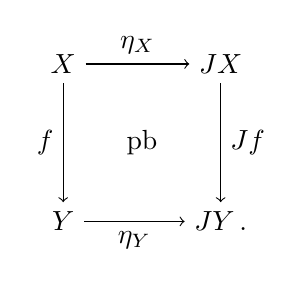
\begin{tikzpicture}
                \node (PB) at (0, 0) {pb};
                \node (X) at (-1, 1) {$X$};
                \node (JX) at (1, 1) {$\mathfrak{J}X$};
                \node (Y) at (-1, -1) {$Y$};
                \node (JY) at (1, -1) {$\mathfrak{J}Y\,.$};
                \draw[->] (X) -- node[above]{$\eta_X$} (JX);
                \draw[->] (Y) -- node[below]{$\eta_Y$} (JY);
                \draw[->] (X) -- node[left]{$f$} (Y);
                \draw[->] (JX) -- node[right]{$\mathfrak{J}f$} (JY);
            \end{tikzpicture}
        \end{gather*}
    }

    \newdef{Super-differential cohesion}{\index{cohesion!super-differential}\index{solid|see{cohesion, super-differential}}
        Consider a differentially cohesive $(\infty,1)$-topos $\mathbf{H}_{\text{bos}}\rightarrow\mathbf{H}_{\text{red}}$. A super-differentially cohesive (or \textbf{solid}\footnote{This terminology stems from the fact that supergeometry is necessary for treating fermions, which are in turn responsible for condensed matter physics and, hence, the study of solid matter.}) topos over $\mathbf{H}_{\text{bos}}$ is a differentially cohesive $(\infty,1)$-topos $\mathbf{H}\rightarrow\mathbf{H}_{\text{red}}$ equipped with an adjoint quadruple $(\mathrm{even}\dashv\iota_{\text{sup}}\dashv\Pi_{\text{sup}}\dashv\mathrm{Disc}_{\text{sup}}):\mathbf{H}\rightarrow\mathbf{H}_{\text{bos}}$ such that $\iota_{\text{sup}}$ (and, hence, also $\mathrm{Disc}_{\text{sup}}$) is fully faithful.

        These structures give the following diagram of $(\infty,1)$-functors (again by uniqueness of adjoints and global sections):
        \begin{gather}
            \label{type:solid_diagram}
            \begin{tikzpicture}[baseline = 0]
                \node (A) at (0, 0) {$\mathbf{H}$};
                \node (B) at (3, 0) {$\mathbf{H}_{\text{bos}}$};
                \node (C) at (6, 0) {$\mathbf{H}_{\text{red}}$};
                \node (D) at (9, 0) {$\infty\mathbf{Grpd}$};
                \node (A1) at (0, 1) {$\phantom{\mathbf{H}}$};
                \node (B1) at (3, 1) {$\phantom{\mathbf{H}_{\text{bos}}}$};
                \node (C1) at (6, 1) {$\phantom{\mathbf{H}_{\text{red}}}$};
                \node (D1) at (9, 1) {$\phantom{\infty\mathbf{Grpd}}$};
                \node (A_1) at (0, -1) {$\phantom{\mathbf{H}}$};
                \node (B_1) at (3, -1) {$\phantom{\mathbf{H}_{\text{bos}}}$};
                \node (C_1) at (6, -1) {$\phantom{\mathbf{H}_{\text{red}}}$};
                \node (D_1) at (9, -1) {$\phantom{\infty\mathbf{Grpd}}$};
                \node (A_2) at (0, -2) {$\phantom{\mathbf{H}}$};
                \node (D_2) at (9, -2) {$\phantom{\infty\mathbf{Grpd}}$};
                \node (A2) at (0, 2) {$\phantom{\mathbf{H}}$};
                \node (B2) at (3, 2) {$\phantom{\mathbf{H}_{\text{bos}}}$};
                \node (C2) at (6, 2) {$\phantom{\mathbf{H}_{\text{red}}}$};
                \node (A3) at (0, 3) {$\phantom{\mathbf{H}}$};
                \node (B3) at (3, 3) {$\phantom{\mathbf{H}_{\text{bos}}}$};
                \draw[left hook->] (B) -- node[above]{$\mathrm{Disc}_{\text{sup}}$} (A);
                \draw[left hook->] (C) -- node[above]{$\mathrm{Disc}_{\text{bos}}$} (B);
                \draw[left hook->] (D) -- node[above]{$\mathrm{Disc}_{\text{red}}$} (C);
                \draw[->] (A1) -- node[above]{$\Pi_{\text{sup}}$} (B1);
                \draw[->] (B1) -- node[above]{$\Pi_{\text{bos}}$} (C1);
                \draw[->] (C1) -- node[above]{$\Pi_{\text{red}}$} (D1);
                \draw[->] (A_1) -- node[above]{$\Gamma_{\text{sup}}$} (B_1);
                \draw[->] (B_1) -- node[above]{$\Gamma_{\text{bos}}$} (C_1);
                \draw[->] (C_1) -- node[above]{$\Gamma_{\text{red}}$} (D_1);
                \draw[left hook->] (D_2) -- node[above]{$\mathrm{coDisc}$} (A_2);
                \draw[left hook->] (B2) -- node[above]{$\iota_{\text{sup}}$} (A2);
                \draw[left hook->] (C2) -- node[above]{$\iota_{\text{bos}}$} (B2);
                \draw[->] (A3) -- node[above]{$\mathrm{even}$} (B3);
            \end{tikzpicture}
        \end{gather}
    }

    \begin{property}[Solid modalities]
        As for cohesive and differentially cohesive topoi, the adjoint functors induce a set of (adjoint) modalities:
        \begin{gather}
            (\rightrightarrows\,\dashv\,\rightsquigarrow\,\dashv\mathrm{Rh}):=(\iota_{\text{sup}}\circ\mathrm{even}\dashv\iota_{\text{sup}}\circ\Pi_{\text{sup}}\dashv\mathrm{Disc}_{\text{sup}}\circ\Pi_{\text{sup}})\,.
        \end{gather}
        These are called the \textbf{fermionic}, \textbf{bosonic} and \textbf{rheonomic} modalities, respectively. Note that, by Diagram~\ref{type:solid_diagram}, a super-differentially cohesive topos also inherits the cohesive and differential modalities.
    \end{property}

    \todo{COMPLETE (e.g.~work by Schreiber)}

\section{Smooth spaces}\index{smooth!space}\label{section:smooth_spaces}

    In this section, some generalizations of spaces that are better behaved when considering their properties as a whole are introduced. Before moving to the smooth setting, a bit of history will be given, starting from the ordinary topological setting.

    The first problem in the study of the global properties of spaces arose in algebraic topology. When consider mapping spaces, it is sometimes useful to use the currying operation
    \begin{gather}
        C(X\times Y,Z)\rightarrow C\bigl(X,C(Y,Z)\bigr)\,.
    \end{gather}
    However, in general, this is not a homeomorphism, i.e.~currying does not define an adjunction and, therefore, $\mathbf{Top}$ is not Cartesian closed (\cref{cat:closed}). This problem was treated by \textit{Steenrod} and others, and the solution was simply to restrict to a smaller class of better behaved spaces: the compactly generated Hausdorff spaces.\footnote{In practice, this is not a problem since all interesting spaces, such as CW complexes, belong to this class.}

    Whilst studying varieties in algebraic geometry, people experienced similar problems. For this reason, \textit{Grothendieck} invented schemes (see \cref{chapter:alggeom} and \cref{section:schemes} in particular). The main takeaway of this approach was that ``it's better to work with a nice category containing some nasty objects, than a nasty category containing only nice objects'' as \textit{Baez} phrases it succinctly.

    The category $\mathbf{Diff}$ of finite-dimensional smooth manifolds suffers the same problems, namely the space of smooth functions $C^\infty(X,Y)$ is, in general, some kind of infinite-dimensional manifold and, hence, cannot be defined internally. It becomes even worse if one studies the mapping spaces between those. \textit{Kriegl} and \textit{Michor} have introduced a framework in which one can work safely, but the main problem with their solution is that not all spaces of interest are included. Certain other operations such as quotients and (co)limits are also not guaranteed to exist within that category.

\subsection{Fr\"olicher spaces}\index{Fr\"olicher space}

    \newdef{Fr\"olicher space}{
        A triple $(X,C_X,F_X)$ consisting of the following data:
        \begin{itemize}
            \item a set $X$,
            \item a set of curves $C_X\subseteq\mathbf{Set}(\mathbb{R},X)$, and
            \item a set of functionals $F_X\subseteq\mathbf{Set}(X,\mathbb{R})$.
        \end{itemize}
        These are required to satisfy the following closure and consistency conditions:
        \begin{enumerate}
            \item For all $c\in C_X$ and $f\in F_X$, the composite is smooth: $f\circ c\in C^\infty(\mathbb{R})$.
            \item If, given $c\in\mathbf{Set}(\mathbb{R},X)$, the composite $f\circ c\in C^\infty(\mathbb{R})$ for all functionals $f\in F_X$, then $c\in C_X$.
            \item If, given $f\in\mathbf{Set}(X,\mathbb{R})$, the composite $f\circ c\in C^\infty(\mathbb{R})$ for all curves $c\in C_X$, then $f\in F_X$.
        \end{enumerate}
        Morphisms of Fr\"olicher spaces are those functions that preserve curves, functionals and smoothness under composition.
    }

    \begin{property}
        The category of Fr\"olicher spaces is bicomplete and Cartesian closed.
    \end{property}

    \newdef{Topology}{\index{topology!curvaceous}\index{topology!functional}
        Consider a Fr\"olicher space $(X,C_X,F_X)$. The \textbf{curvaceous topology} on $X$ is the final topology with respect to the curves $C_X$. The \textbf{functional topology} on $X$ is the initial topology with respect to the functionals $F_X$.
    }

    \todo{COMPLETE (e.g. Isbell enveloppe / duality)}

\subsection{Smooth sets}

    \newdef{Concrete site}{\index{concrete!site}
        Consider a site $(\mathbf{C},J)$. It is said to be concrete if
        \begin{enumerate}
            \item the functor $\mathbf{C}(\ast,-):\mathbf{C}\rightarrow\mathbf{Set}$ is faithful, and
            \item for every covering family $\{f_i:U_i\rightarrow U\}_{i\in I}\in J(U)$, the morphism
            \begin{gather}
                \bigsqcup_{i\in I}\mathbf{C}(\ast,f_i):\bigsqcup_{i\in I}\mathbf{C}(\ast,U_i)\rightarrow\mathbf{C}(\ast,U)
            \end{gather}
            is surjective.
        \end{enumerate}
    }

    \newdef{Concrete presheaf}{\index{concrete!sheaf}
        Consider a concrete site $(\mathbf{C},J)$. For every presheaf $X\in\mathbf{Psh}(\mathbf{C})$ and object $U\in\ob{C}$, denote by
        \begin{gather}
            X_U:X(U)\rightarrow\mathbf{Set}\bigl(\mathbf{C}(\ast,U),X(\ast)\bigr)
        \end{gather}
        the adjunct of the restriction morphism
        \begin{gather}
            X(U)\times\mathbf{C}(\ast,U)\rightarrow X(\ast)\,.
        \end{gather}
        The presheaf $X$ is said to be concrete if, for each $U\in\ob{C}$, the map $X_U$ is injective. This says that concrete presheaves are subobjects of presheaves of the form
        \begin{gather}
            U\mapsto\mathbf{Set}\bigl(\mathbf{C}(\ast,U),X(\ast)\bigr)\,.
        \end{gather}
        This definition also agrees with \cref{topos:concrete_object}.
    }

    \begin{property}
        The category of sheaves on a concrete site is a local topos (\cref{topos:local_topos}). The right adjoint $\func{\mathrm{coDisc}}{Set}{H}$ sends a set $A$ to the functor $U\mapsto\mathbf{Set}\bigl(\mathbf{C}(\ast,U),A\bigr)$.
    \end{property}
    This property allows to define concrete objects in any local topos in an alternative way (by slightly modifying \cref{topos:characterization_embedding} to allow for separation instead of locality).
    \newdef{Concrete object}{\index{concrete!object}
        Consider a local geometric morphism $\Gamma:\mathbf{H}\rightarrow\mathcal{S}$. Consider the class $V$ of local isomorphisms with respect to $\Gamma$. An object in $\mathbf{H}$ is said to be concrete if it is $V$-separated, i.e.~its Yoneda embedding maps morphisms in $V$ to monos.
    }
    \begin{remark}
        Note that concrete sheaves carry two kinds of sheaf-theoretic information. On the one hand they are actual sheaves with respect to the Grothendieck topology of the underlying site and, on the other hand, they are separated presheaves with respect to the topology generated by global elements $\ast\rightarrow U$.
    \end{remark}

    \begin{property}[Concretification]\label{topos:concretification}
        Consider a local 1-topos $\mathbf{H}$.\footnote{The restriction to ordinary topoi ensures that ordinary image factorization suffices. For higher topoi, this would not be the case and higher image factorizations would be required.} Every topos has an epi/mono factorization giving rise to the image $\im(f)$ of a morphism $f\in\hom(\mathbf{H})$. The concretification of an object $X\in\ob{H}$ is given by the image $\im(\eta^\sharp_X)$. 
    \end{property}

    In the case of the site of Cartesian spaces, the following notion is obtained.
    \newdef{Diffeological space}{\index{diffeology}
        A diffeology on a set $X$ is a concrete sheaf $\mathcal{D}_X$ on $\mathbf{CartSp_{\text{diff}}}$ such that $\Gamma\mathcal{D}_X=X$.
    }

    \newadef{Diffeological space}{\index{diffeology}\index{plot}
        Let $X$ be a set. A diffeology $\mathcal{D}_X$ on $X$ is defined as a collection of functions $f:U\subseteq\mathbb{R}^n\rightarrow X$, called \textbf{plots}, satisfying the following conditions (where $U,V$ and $W$ are open sets):
        \begin{enumerate}
            \item $\mathcal{D}_X$ contains all constant functions.
            \item If $\{U_i\}_{i\in I}$ is an open cover of $U$ and if $f|_{U_i}\in\mathcal{D}_X$ for all $i\in I$, then $f\in\mathcal{D}_X$.
            \item If $f\in\mathcal{D}_X$ and $g:W\subseteq\mathbb{R}^m\rightarrow\dom(f)$ is smooth, then $f\circ g\in\mathcal{D}_X$.
        \end{enumerate}
        The set $X$ can be turned into a topological space by equipping it with the \textbf{$\mathcal{D}_X$-topology}, the final topology with respect to $\mathcal{D}_X$.
    }
    \remark{Note that, in contrast to ordinary manifolds, the plots in a diffeology can have domains of different dimensions.}

    \newdef{Smooth map}{\index{smooth!function}
        Let $\mathcal{D}_X$ and $\mathcal{D}_Y$ be diffeological spaces. A map $g:X\rightarrow Y$ is said to be smooth if $g\circ f\in\mathcal{D}_Y$ for all $f\in\mathcal{D}_X$. The diffeological spaces together with their differentiable morphisms form a category $\mathbf{DiffSp}$.
    }

    \newdef{Chen space}{\index{Chen space}
        If the open sets in the definition of a diffeological space are replaced by convex sets, the notion of smooth spaces due to \textit{Chen} is obtained.
    }

    \begin{adefinition}[Manifold]\index{manifold}
        A diffeological space that is locally diffeomorphic to a Euclidean space. A map between manifolds is smooth in the diffeological sense if and only if it smooth in the sense of \cref{manifolds:smooth_function}.
    \end{adefinition}

    There exist two trivial smooth structures.
    \begin{example}[Discrete structure]\index{discrete!smooth structure}
        The minimal smooth structure, i.e.~the one obtained by taking the plots to be the constant functions.
    \end{example}
    \begin{example}[Indiscrete structure]
        The maximal smooth structure, i.e.~the one obtained by taking all functions to be plots.
    \end{example}

    The notion of diffeological spaces can be further generalized by passing to the full sheaf topos on Cartesian spaces.
    \newdef{Smooth set}{\index{smooth!set}\index{Nullstellensatz}
        \begin{gather}
            \mathbf{SmoothSet}:=\mathbf{Sh(CartSp_{\text{diff}})}
        \end{gather}
        The topology on this site is generated by the coverage of differentiably good covers (\cref{manifold:good_cover}). In fact, this topology coincides with the usual one consisting of open covers. The category of smooth sets is also denoted by $\mathbf{C^\infty}$.

        To phrase this in the sense of \cref{section:cohesion}, smooth sets form a cohesive topos over $\mathbf{Set}$, where $\mathrm{Disc}$ and $\mathrm{coDisc}$ assign the discrete and codiscrete structures from the preceding examples, respectively. Moreover, this cohesive topos satisfies the \textit{Nullstellensatz}~\ref{topos:nullstellensatz}.
    }

    \begin{property}
        There exists an adjunction
        \begin{gather}
            \mathbf{Top}\adj{\mathrm{top}}{\mathrm{diff}}\mathbf{C^\infty}\,.
        \end{gather}
        The right adjoint endows a topological space $X$ with the smooth structure for which every continuous map $U\rightarrow X$ is a plot. Its left adjoint sends a smooth space to the topological space equipped with the finest topology for which all plots become continuous maps.
    \end{property}

    \begin{property}\label{topos:discrete_smooth_sets}
        The adjunction $\Pi_0\dashv\mathrm{Disc}$ exhibits the discrete smooth sets, i.e.~the constant sheaves, as the reflective subcategory on $\mathbb{R}$-local objects (see also \cref{model:reflective_localization}).
    \end{property}

    As noted above, the subcategory of diffeological spaces exactly consists of the concrete smooth sets, i.e.~those smooth sets that have an underlying set of points. A common example of smooth sets that do not have such an underlying set is given by de Rham spaces.
    \begin{example}[Differential forms]\index{moduli space!of differential forms}
        Consider the $k^{\text{th}}$ de Rham functor $\Omega^k$ on the category $\mathbf{Diff}$. This functor assigns to every smooth manifold its space of differential $k$-forms. Locally defined forms can be glued together if they agree on intersections, i.e.~they satisfy the sheaf condition. This shows that $\Omega^k$ defines a smooth set, albeit one that is far from an ordinary smooth manifold. It is called the \textbf{(universal) moduli space of differential $k$-forms}. Note, however, that for a given smooth set $X\in\mathbf{C^\infty}$, the plots of $[X,\Omega^k]$ correspond to differential $k$-forms on the product $\mathbb{R}^n\times X$ and not to $\mathbb{R}^n$-parametrized forms on $X$. For the latter, one should consider the concretification $\mathrm{conc}[X,\Omega^k]$.

        One can go even further and characterize specific geometric structures in terms of this functor. Consider for example the subfunctor $\Omega^2_{\text{cl}}$ that assigns closed two-forms to a manifold. This also defines a smooth space and, hence, one can consider the slice category $\mathbf{C^\infty}/\Omega^2_{\text{cl}}$. It is not hard to show that the category $\mathbf{SpMfd}$ of symplectic manifolds admits an embedding into this slice category.
    \end{example}
    \begin{property}[Universal differential forms]
        Consider the differential $n$-form
        \begin{gather}
            \omega_{\text{univ}}\in\Omega^n(\Omega^n)
        \end{gather}
        modulated by the identity morphism on $\Omega^n$, the universal differential $n$-form. Every differential $n$-form, on any smooth set, can be obtained as a pullback of $\omega_{\text{univ}}$.
    \end{property}

    \begin{example}[Path space]\index{path!space}
        Since every topos is Cartesian closed, all internal homs exist. The path space of a smooth set $X$ is defined as
        \begin{gather}
            \mathbf{P}X := [\mathbb{R},X]\,.
        \end{gather}
        Its underlying set is given by the set of smooth plots (trajectories): $\Gamma[\mathbb{R},X]\cong\mathbf{C^\infty}(\mathbb{R},X)$.
    \end{example}

    Analogously, the internal hom out of $X$ gives the moduli space of smooth functions on $X$:
    \begin{gather}
        \mathbf{C^\infty}(X) := [X,\mathbb{R}]\,.
    \end{gather}

    \newdef{Transgression}{\index{transgression}
        Consider a smooth set $X\in\ob{C^\infty}$. Transgression of differential forms on $X$ along a compact $k$-manifold $\Sigma$ is defined as the composite:
        \begin{gather}
            \tau_\Sigma\omega := \Int_\Sigma[\Sigma,\omega]:[\Sigma,X]\rightarrow[\Sigma,\Omega^n]\xrightarrow{\int_\Sigma}\Omega^{n-k}\,.
        \end{gather}
        An alternative approach uses a pullback along the evaluation morphism $\mathrm{ev}_\Sigma:\Sigma\times[\Sigma,X]\rightarrow X$.
    }
    \begin{property}
        If the compact $k$-manifold $\Sigma$ has a boundary, transgression of closed differential forms along $\Sigma$ and $\partial\Sigma$ is related by the de Rham differential:
        \begin{gather}
            \tau_{\partial\Sigma}(\omega) = (-1)^{k+1}\dr\tau_\Sigma\omega
        \end{gather}
        for all $\omega:X\rightarrow\Omega^n_{\text{cl}}$.
    \end{property}

\subsection{Smooth algebras}

    \newdef{Smooth algebra}{\index{smooth!algebra}
        For any smooth manifold $M$, the algebra of smooth functions can be obtained as a hom-object:
        \begin{gather}
            C^\infty(M):=C^\infty(M,\mathbb{R})=\mathbf{Diff}(M,\mathbb{R})\,.
        \end{gather}
        Since hom-functors are (finite) product-preserving, the multiplication $C^\infty(M)\times C^\infty(M)\rightarrow C^\infty(M)$ can be seen to be induced by the multiplication on $\mathbb{R}$:
        \begin{gather}
            C^\infty(M,\mathbb{R}\times\mathbb{R})\cong C^\infty(M)\times C^\infty(M)\,.
        \end{gather}
        Furthermore, the hom-functor is covariant in the second argument and, hence, defines a copresheaf on the category $\mathbf{CartSp_{\text{diff}}}$. Generalizing this situation, smooth algebras are defined as finite product-preserving copresheaves on $\mathbf{CartSp_{\text{diff}}}$. This (functor) category is denoted by $\mathbf{C^\infty Alg}$.
    }
    \newdef{Underlying algebra}{
        Given a smooth algebra $R\in\mathbf{C^\infty Alg}$, its underlying algebra $U(R)$ is defined as the set $R(\mathbb{R})$ equipped with the canonically induced ring operations.
    }

    \newdef{Finitely generated smooth algebra}{
        Since ordinary $R$-algebras are finitely generated if and only if they are of the form $R[x_1,\ldots,x_k]/I$ for some integer $k\in\mathbb{N}$ and some ideal $I$, a smooth algebra is said to be finitely generated if it is of the form $C^\infty(\mathbb{R}^n)/I$ for some $n\in\mathbb{N}$ and some ideal $I$ in the underlying algebra.
    }
    \newdef{Smooth locus}{\index{smooth!locus}
        Let $\mathbf{C^\infty Alg^{fin}}$ denote the category of finitely generated smooth algebras. The category of \textbf{smooth loci} is defined as $(\mathbf{C^\infty Alg^{fin}})^{\text{op}}$. The smooth locus corresponding to a smooth algebra $R$ is often denoted by $\ell R$.
    }

\subsection{Supergeometry}

    In this section, the definition of smooth spaces (and sets) is generalized to the odd (fermionic) sector, i.e.~`super smooth sets' will be defined. This gives an explicit example of a super-differentially cohesive $(\infty,1)$-topos.

    \newdef{Superscheme}{\index{super-!scheme}
        The category of affine superschemes is defined as the opposite of the category of supercommutative superalgebras, the commutative monoids internal to $\mathbf{sVect}$:
        \begin{gather}
            \mathbf{Aff(sVect)} := \mathbf{sCAlg}^{\text{op}} := \mathbf{CMon(sVect)}\,.
        \end{gather}
        More generally, one can define affine schemes internal to any symmetric monoidal category.
    }

    \newdef{Infinitesimally thickened space}{\index{thickened space}\index{Weil!algebra}\index{Artin!algebra}\label{hdg:infinitesimal_thickening}
        First, consider a point $\mathbb{R}^0$. Its infinitesimal thickening should be a space such that every function that vanishes at the origin is actually nilpotent (this is essentially a version of the Kock--Lawvere axiom~\ref{synth:kock_lawvere_axiom}):
        \begin{gather}
            \mathbb{D} := \mathrm{Spec}(A)\,,
        \end{gather}
        where $A:=\mathbb{R}\oplus V$ for $V$ a finite-dimensional nilpotent ideal.\footnote{Algebras of this form are also called \textbf{Weil algebras} or \textbf{local Artin algebras}.} A Euclidean space can be infinitesimally thickened by taking the product with $\mathbb{D}$ or, at the algebraic level, by taking the tensor product with $A$. A morphism of such spaces is defined by an $\mathbb{R}$-algebra morphism between their associated algebras. These form the category $\mathbf{FormalCartSp_{\text{diff}}}$.
    }
    \newdef{Superpoint}{\index{super-!point}\index{super-!space}
        A space of the form $\mathrm{Spec}(\Lambda^\bullet\mathbb{R}^n)$. This is often denoted by $\mathbb{R}^{0\mid n}$. The \textbf{super-Euclidean space} $\mathbb{R}^{m\mid n}$ is obtained as the product of an ordinary Euclidean space $\mathbb{R}^m$ and the superpoint $\mathbb{R}^{0\mid n}$, i.e.~its algebra of smooth functions is $C^\infty(\mathbb{R}^m)\otimes\Lambda^\bullet\mathbb{R}^n$.\footnote{Compare this to the definition of supermanifolds (\cref{hdg:supermanifold}).}
    }
    \begin{example}[First-order neighbourhood]\index{neighbourhood}
        For $A=\mathbb{R}[\varepsilon]/\varepsilon^2$, the definition of an infinitesimal thickening recovers the first-order infinitesimal neighbourhood of \cref{synth:infinitesimal_line}:
        \begin{gather}
            \mathbb{D}^1:=\mathrm{Spec}(\mathbb{R}[\varepsilon]/\varepsilon^2)\,.
        \end{gather}
        The morphism dual to the mapping implied by the Kock--Lawvere axiom~\ref{synth:kock_lawvere_axiom} gives an inclusion map $\mathbb{D}^1\hookrightarrow\mathbb{R}^1$. (This example can easily be generalized to $k^{\text{th}}$-order neighbourhoods.) This algebra is the algebra of functions on the even part of the superplane:
        \begin{gather}
            \mathcal{O}\bigl(\mathrm{even}\,\mathbb{R}^{0\mid 2}\bigr)\cong\mathbb{R}[\varepsilon]/\varepsilon^2\,.
        \end{gather}
    \end{example}

    \begin{property}[Morphisms]
        First, consider the morphisms from a Euclidean space into an infinitesimal neighbourhood $\mathbb{D}^k$. Since such morphisms are dual to algebra morphisms, one should consider morphisms of the form $\mathbb{R}[\varepsilon]/\varepsilon^{k+1}\rightarrow C^\infty(\mathbb{R}^n)$. However, being an algebra morphism implies that $f(1)=1$ and that nilpotents are mapped to nilpotents. The algebra of smooth functions on a Euclidean space does not contain nilpotents and, hence, there exists a unique function into an infinitesimal neighbourhood (the one that factorizes through the one-point set).

        For morphisms out of (first-order) infinitesimal neighbourhoods, one obtains the property, known from synthetic geometry, that morphisms of the form $\mathbb{R}^n\times\mathbb{D}^1\rightarrow\mathbb{R}^n$ correspond to vector fields on $\mathbb{R}^n$ exactly when the postcomposition with the inclusion $\mathbb{R}^n\hookrightarrow\mathbb{R}^n\times\mathbb{D}^1$ is the identity.
    \end{property}

    \newdef{Formal smooth set}{\index{formal!set}\index{smooth|seealso{formal}}\index{topos!Cahiers}\index{plot}
        A sheaf on the site of infinitesimally thickened Euclidean spaces, where covers are of the form $\{U_i\times\mathrm{Spec}(A)\mid U_i\subseteq\mathbb{R}^n\}$, for $A$ a commutative (hence, even) algebra. The category of formal smooth sets or, equivalently, the sheaf topos on $\mathbf{FormalCartSp_{diff}}$ is also called the \textbf{Cahiers topos}. The sets in the image of a formal smooth set $X$ are called the sets of \textbf{plots} of $X$ and can be interpreted as sets of functions into $X$ (in analogy with the definition of smooth sets).
    }

    \newdef{Super smooth set}{\index{smooth!set}\index{topos!Dubuc}
        By combining infinitesimal thickenings and superpoints, the category $\mathbf{SuperFormalCartSp_{diff}}$ is obtained. A sheaf on this category is called a super smooth set. Since \textit{Dubuc} introduced the Cahiers topos, the category of super smooth sets is sometimes called the \textbf{super-Dubuc topos}.
    }

    \begin{property}[Cohesion]
        The full subcategory inclusion $\mathbf{CAlg}\hookrightarrow\mathbf{sCAlg}$ is part of an adjoint cylinder, where the left and right adjoints are given by projection onto the even part and quotienting out the odd part:
        \begin{gather}
            \mathrm{even}\dashv\,\iota\dashv-/(-)_{\text{odd}}\,,
        \end{gather}
        where $(-)_{\text{odd}}$ indicates that the ideal generated by odd elements is quotiented out, i.e.~every term containing at least one odd factor is set to zero. These define canonical functors, $\mathrm{even}$ and $\Pi_{\text{sup}}$, from the category of affine superschemes to affine schemes (and, hence, also between the larger categories of superschemes and schemes). Moreover, the inclusion of affine schemes into infinitesimally thickened spaces also admits a right adjoint given by reduction: $\Pi_{\text{inf}}(\mathbb{R}^n\times\mathbb{D}):=\mathbb{R}^n$.

        These, in turn, induce a system of ajunctions between the sheaf topos of smooth sets, the Cahiers topos and the super-Dubuc topos, characterizing them as a cohesive, elastic and solid topoi, respectively:
        \begin{gather}
            \begin{tikzpicture}[baseline = 0]
                \node[align=center] (A) at (0, 0) {\textbf{Super}\\\textbf{Smooth}\\\textbf{Set}};
                \node[align=center] (B) at (4, 0) {\textbf{Formal}\\\textbf{Smooth}\\\textbf{Set}};
                \node (C) at (8, 0) {$\mathbf{C^\infty}$};
                \node (D) at (12, 0) {$\mathbf{Set}$};
                \node (A1) at (0, 1) {$\phantom{\mathbf{H}}$};
                \node (B1) at (4, 1) {$\phantom{\mathbf{H}_{\text{bos}}}$};
                \node (C1) at (8, 1) {$\phantom{\mathbf{H}_{\text{red}}}$};
                \node (D1) at (12, 1) {$\phantom{\infty\mathbf{Grpd}}$};
                \node (A_1) at (0, -1) {$\phantom{\mathbf{H}}$};
                \node (B_1) at (4, -1) {$\phantom{\mathbf{H}_{\text{inf}}}$};
                \node (C_1) at (8, -1) {$\phantom{\mathbf{H}_{\text{red}}}$};
                \node (D_1) at (12, -1) {$\phantom{\infty\mathbf{Grpd}}$};
                \node (A_2) at (0, -2) {$\phantom{\mathbf{H}}$};
                \node (D_2) at (12, -2) {$\phantom{\infty\mathbf{Grpd}}$};
                \node (A2) at (0, 2) {$\phantom{\mathbf{H}}$};
                \node (B2) at (4, 2) {$\phantom{\mathbf{H}_{\text{inf}}}$};
                \node (C2) at (8, 2) {$\phantom{\mathbf{H}_{\text{red}}}$};
                \node (A3) at (0, 3) {$\phantom{\mathbf{H}}$};
                \node (B3) at (4, 3) {$\phantom{\mathbf{H}_{\text{inf}}}$};
                \draw[left hook->] (B) -- node[above]{$\mathrm{Disc}_{\text{sup}}$} (A);
                \draw[left hook->] (C) -- node[above]{$\mathrm{Disc}_{\text{inf}}$} (B);
                \draw[left hook->] (D) -- node[above]{$\mathrm{Disc}_{\text{red}}$} (C);
                \draw[->] (A1) -- node[above]{$\Pi_{\text{sup}}$} (B1);
                \draw[->] (B1) -- node[above]{$\Pi_{\text{inf}}$} (C1);
                \draw[->] (C1) -- node[above]{$\Pi_{\text{red}}$} (D1);
                \draw[->] (A_1) -- node[above]{$\Gamma_{\text{sup}}$} (B_1);
                \draw[->] (B_1) -- node[above]{$\Gamma_{\text{inf}}$} (C_1);
                \draw[->] (C_1) -- node[above]{$\Gamma_{\text{red}}$} (D_1);
                \draw[left hook->] (D_2) -- node[above]{$\mathrm{coDisc}$} (A_2);
                \draw[left hook->] (B2) -- node[above]{$\iota_{\text{sup}}$} (A2);
                \draw[left hook->] (C2) -- node[above]{$\iota_{\text{inf}}$} (B2);
                \draw[->] (A3) -- node[above]{$\mathrm{even}$} (B3);
            \end{tikzpicture}
        \end{gather}
        The top four functors in every column are obtained by Kan extension from the functors between affine spaces (\cref{cat:kan_quadruple}). The others follow from uniqueness and composition properties of adjoints and the fact that the coverages on $\mathbf{SuperSmoothSet}$ and $\mathbf{FormalSmoothSet}$ are trivial along infinitesimal thickenings and odd dimensions.
    \end{property}

    By the general theory of cohesive topoi, the diagram of adjunctions induce a another diagram of adjoint modalities. These are listed below.
    \newdef{Fermionic modalities}{
        The adjoint cylinder induced by the inclusion $\mathbf{CAlg}\hookrightarrow\mathbf{sCAlg}$ in turn gives rise to the adjoint modalities
        \begin{gather}
            \overrightarrow{\overrightarrow{(-)}}\dashv\overset{\rightsquigarrow}{(-)}\,.
        \end{gather}
        The left adjoint sends a super smooth set to its `bifermionic' space, where only paired fermions occur. The right adjoint sends a super smooth set to its underlying bosonic space and might, therefore, be called the \textbf{bosonic modality}.

        Moreover, since these modalities come from an adjoint quadruple, a further right adjoint exists. The rheonomy modality corresponds to localization at the superpoint:
        \begin{gather}
            \mathrm{Rh}\cong L_{\mathbb{R}^{0\mid1}}\,,
        \end{gather}
        akin to \cref{topos:discrete_smooth_sets}.
    }

    The following definition is dual to \cref{algebra:reduction}.
    \newdef{Reduction}{\index{reduction}\index{infinitesimal}
        By \cref{topos:differential_modalities}, $\mathbf{SuperSmoothSet}$ admits differential modalities to both $\mathbf{FormalSmoothSet}$ and $\mathbf{SmoothSet}$. The reduction modality $\mathfrak{R}$ simply drops all infinitesimal directions, both even- and odd-graded:
        \begin{gather}
            \mathfrak{R}(\mathbb{R}^{m\mid n}\times\mathbb{D}) = \mathbb{R}^m\,.
        \end{gather}

        The \textbf{infinitesimal neighbourhood} (to arbitrary order) of a formal smooth subset $Y\hookrightarrow X$ is defined by taking its plots to be those plots of $X$ for which the reductions factorize through plots of $Y$.
    }
    \newdef{Shape modality}{\index{modality|seealso{shape}}\index{shape}\index{de Rham|seealso{shape}}
        The \textbf{(infinitesimal) shape} or \textbf{de Rham shape} $\mathfrak{J}X$ of a super smooth set $X$ is given, throught duality/adjointness, by the super smooth set obtained by reducing the plots of $X$:
        \begin{gather}
            \mathfrak{J}X(U) := X(\mathfrak{R}(U))\,.
        \end{gather}
        This construction identifies all infinitesimally close points.
    }

    \newdef{Tangent bundle}{\index{tangent!bundle}
        Consider a super smooth set $X$. Its tangent bundle is given by the internal hom out of the infinitesimal disk:
        \begin{gather}
            TX := [\mathbb{D}^1,X]\,.
        \end{gather}
        Precomposition by the unique global element of $\mathbb{D}^1$ gives the bundle projection $TX\rightarrow X$. Analogously, the internal hom out of the superpoint gives the odd tangent bundle (see also Definition~\ref{hdg:odd_tangent_bundle}):
        \begin{gather}
            \Pi TX := [\mathbb{R}^{0\mid1},X]\,.
        \end{gather} 
    }


    \newdef{Local diffeomorphism\footnotemark}{\index{local!diffeomorphism}
        Recall \cref{topos:formally_etale}. In the setting of super smooth sets, this is equivalent to a morphism $f:X\rightarrow Y$ such that the thickened plots of $X$ can be identified with those of $Y$ whose reduction comes from a Euclidean plot of $X$. Equivalently, by taking internal homs, a morphism of super smooth sets is formally \'etale if and only if
        \begin{gather*}
            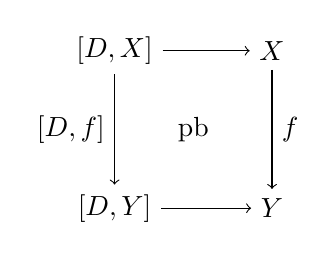
\begin{tikzpicture}
                \node (PB) at (0, 0) {pb};
                \node (X) at (-1, 1) {$[\mathbb{D},X]$};
                \node (JX) at (1, 1) {$X$};
                \node (Y) at (-1, -1) {$[\mathbb{D},Y]$};
                \node (JY) at (1, -1) {$Y$};
                \draw[->] (X) -- (JX);
                \draw[->] (Y) -- (JY);
                \draw[->] (X) -- node[left]{$[\mathbb{D},f]$} (Y);
                \draw[->] (JX) -- node[right]{$f$} (JY);
            \end{tikzpicture}
        \end{gather*}
        is a pullback square for all infinitesimally thickened (super)points. By taking $\mathbb{D}=\mathbb{D}^1$, the Inverse Function Theorem~\ref{bundle:inverse_function_theorem} can be recovered.

        This can also be related to the definition in commutative algebra (and dually, that in algebraic geometry) as follows. The shape modality is right adjoint to the reduction modality. Sending a ring (extension) to its representable presheaf and using the Yoneda lemma gives the diagram
        \begin{gather*}
            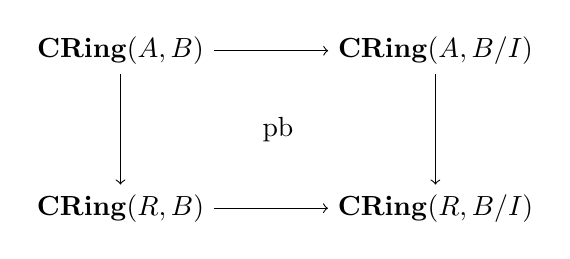
\begin{tikzpicture}
                \node (PB) at (0, 0) {pb};
                \node (X) at (-2, 1) {$\mathbf{CRing}(A,B)$};
                \node (JX) at (2, 1) {$\mathbf{CRing}(A,B/I)$};
                \node (Y) at (-2, -1) {$\mathbf{CRing}(R,B)$};
                \node (JY) at (2, -1) {$\mathbf{CRing}(R,B/I)$};
                \draw[->] (X) -- (JX);
                \draw[->] (Y) -- (JY);
                \draw[->] (X) -- (Y);
                \draw[->] (JX) -- (JY);
            \end{tikzpicture}
        \end{gather*}
        This square being a pullback exactly corresponds to the lifting condition in \cref{algebra:formally_etale}.
    }

    \begin{property}\label{hdg:bosonic_formally_etale}
        Local diffeomorphisms are preserved by the bosonic modality. If $f$ is formally \'etale, so is $\overset{\rightsquigarrow}{f}$.
    \end{property}

    \newadef{Smooth manifold}{\index{manifold}
        A diffeological space (in its incarnation as a formal smooth set) equipped with a family of local diffeomorphisms from Euclidean spaces (also regarded as formal smooth sets) such that every point of the space lies in the image of at least one such morphism (and such that the final topology induced by the plots of the smooth set is paracompact Hausdorff).
    }

    \newdef{$V$-manifold}{
        Consider a group object $V$ in $\mathbf{SuperSmoothSet}$. A $V$-manifold is a super smooth set $X$ equipped with a span
        \begin{gather*}
            \begin{tikzpicture}
                \node (U) at (0, 0) {$U$};
                \node (V) at (-2, -2) {$V$};
                \node (X) at (2, -2) {$X$};
                \draw[->] (U) -- node[above left]{\'et} (V);
                \draw[->] (U) -- node[above right]{\'et, epi} (X);
            \end{tikzpicture}
        \end{gather*}
    }
    \newdef{Supermanifold}{\index{super-!manifold}
        A supermanifold of \textbf{(super)dimension} $(m\mid n)$ is a super smooth set $X$ equipped with a formally \'etale epimorphism $\sqcup_{i\in I}\mathbb{R}^{m\mid n}\rightarrow X$ for some index set $I$.

        Using the notion of supermanifold, one can also define super fibre bundles (and other common notions from differential geometry). Given such a bundle $E\rightarrow M$, its (super)space of sections is the fibre product
        \begin{gather*}
            \Gamma(E) := [M,E]\times_{[M,M]}\mathcal{Y}\{\mathbbm{1}_M\}\,.
        \end{gather*}
    }

    \begin{property}
        By \cref{hdg:bosonic_formally_etale} above, the bosonic space underlying a $V$-manifold is a $\overset{\rightsquigarrow}{V}$-manifold.
    \end{property}

\section{Higher Lie theory}

    In this section, some notions about groups, Lie groups and groupoids (\namecrefs{section:groups}~\ref{section:groups}, \ref{section:lie_groups} and~\ref{section:groupoids}) are extended to the setting of higher category theory.

\section{\difficult{Gauge theory}}

    Recall the notions of \cref{chapter:topos}, in particular the notions of stacks and higher topoi. The $(\infty,1)$-category of smooth $\infty$-stacks can be described in terms of the (left Bousfield) localization of a suitable presheaf category by Lurie's theorem~\ref{model:lurie_presentation}.

    The first possibility is the category of $\infty$-presheaves on $\mathbf{Diff}$ with the localization at open covers. The second possibility is the dense subsite $\mathbf{CartSp_{\text{diff}}}$ with localization at good open covers. Both will result in a \v{C}ech model structure (\cref{topos:cech_model_structure}). However, the specific properties will differ.

    \begin{example}[Classifying stacks]
        Consider the example of a Lie group $G$ and its classifying stack $\mathbf{B}G$. In the first model structure, the mapping space $\mathbf{H}(M,\mathbf{B}G)$, for $M$ a smooth manifold, is simply presented\footnote{This means the homotopy-invariant hom-object in the underlying presheaf category, where the domain is replaced by a cofibrant object and the codomain by a fibrant object.} by $\hom(M,\mathbf{B}G)$, since $M$ is cofibrant as a representable presheaf and $\mathbf{B}G$ is fibrant by gluing over covers. So, mapping spaces $\mathbf{H}(M,\mathbf{B}G)$ are just given by groupoids of $G$-bundles over $M$.

        On the subsite $\mathbf{CartSp}_{\text{diff}}$, the presheaves represented by manifolds are not cofibrant anymore. However, \v{C}ech nerves of open covers give a cofibrant replacement. On the other hand, over Cartesian spaces, the stacks are trivial and can be presented as action groupoids $\ast/\!\!/G$ (the ordinary deloopings). A fibrant replacement is given by the presheaf
        \begin{gather}
            U\mapsto N_\Delta\bigl(\ast/\!\!/C^\infty(U,G)\bigr)\,.
        \end{gather}
        This presheaf is also equivalent to the groupoid of $G$-bundles (over $U$). The derived mapping space in this situation is given by (normalized) $G$-valued \v{C}ech cocycles.
    \end{example}

\subsection{Lie groupoids}

    \newdef{Lie groupoid\footnotemark}{\index{Lie!groupoid}\label{hdg:lie_groupoid}
        \footnotetext{In a similar way one could define \textit{topological groupoids, \'etal\'e groupoids}, ...}
        A groupoid internal to $\mathbf{Diff}$.
    }
    \begin{remark}
        Note that \cref{cat:internal_category} requires the existence of pullbacks. In the category $\mathbf{Diff}$, this is equivalent to assuming that the source and target morphisms are (surjective) submersions.

        In the Ehresmannian approach, the manifold of composable morphisms $D_1\times_{D_0}D_1$ is given as part of the data. Hence, no further assumptions have to be made about the source and target morphisms.
    \end{remark}

    \newdef{Lie algebroid}{\index{Lie!algebroid}\index{anchor}\label{hdg:lie_algebroid}
        A vector bundle $\pi:E\rightarrow M$ together with a morphism $\rho:E\rightarrow TM$, called the \textbf{anchor map}, and a Lie bracket on $\Gamma(E)$ such that the following Leibniz-type property is satisfied:
        \begin{gather}
            [X,fY] = f[X,Y] + \rho(X)(f)Y\,.
        \end{gather}
        This property also implies that $\rho$ preserves the Lie bracket:
        \begin{gather}
            \rho([X,Y]) = [\rho(X),\rho(Y)]\,.
        \end{gather}
        In local coordinates $x^i$ and for a local basis of sections $s_\alpha$, the bracket and anchor can be expressed in terms of structure functions:
        \begin{gather}
            \begin{aligned}
                \rho(s_\alpha) &= R^i_\alpha\partial_i\,,\\
                [s_\alpha,s_\beta] &= C^\gamma_{\alpha\beta}(x)s_\gamma\,.
            \end{aligned}
        \end{gather}
        The Lie algebroid properties then imply the following conditions on these structure functions:
        \begin{gather}
            R^j_\alpha\pderiv{R^i_\beta}{x^j}-R^j_\beta\pderiv{R^i_\alpha}{x^j} = R^i_\gamma C^\gamma_{\alpha\beta}
        \end{gather}
        and
        \begin{gather}
            R^i_\alpha\pderiv{C^\kappa_{\beta\gamma}}{x^i}+C^\kappa_{\alpha\mu}C^\mu_{\beta\gamma} + (\alpha\leftrightarrow\beta\leftrightarrow\gamma) = 0\,.
        \end{gather}
    }

    \begin{example}[Tangent Lie algebroid]\index{pair!groupoid}
        The tangent bundle over a smooth manifold is a Lie algebroid with $\rho=\mathbbm{1}_{TM}$.

        Consider the \textbf{pair groupoid} or \textbf{codiscrete groupoid} $\mathbf{M\times M}$:
        \begin{itemize}
            \item\textbf{Objects}: $M$, and
            \item\textbf{Morphisms}: $M\times M$, i.e.~between every two points there exists a unique morphism.
        \end{itemize}
        Both the fundamental groupoid $\symbf{\Pi}_1(M)$ of \cref{topology:fundamental_groupoid} and the pair groupoid $\mathbf{M\times M}$ \textit{integrate} the tangent Lie algebroid.
    \end{example}

    \todo{ADD LIE INTEGRATION OF ALGEBROIDS}

    One can generalize the dual construction of $L_\infty$-algebras even further.
    \newdef{$L_\infty$-algebroid}{\label{hdg:l_infty_algebroid}
        Consider \cref{hda:l_infinity_bis} of the Chevalley--Eilenberg algebra for an $L_\infty$-algebra. By replacing the base field by a smooth algebra $C^\infty(M)$ for some smooth manifold $M$ and the (graded) vector space $V$ by a module of sections $\Gamma(E)$ of a (graded) vector bundle $E\rightarrow M$, one obtains the notion of a $L_\infty$-algebroid.
    }
    \begin{property}
        $L_\infty$-algebras can be recovered by considering the special case $M=\{\ast\}$.
    \end{property}

    \begin{example}[de Rham complex]\index{de Rham!complex}
        Consider the tangent algebroid of a smooth manifold $M$. The associated Chevalley--Eilenberg complex is equivalent to the de Rham complex $\Omega^\bullet(M)$.
    \end{example}

\section{Weak groups}

    \newdef{Weak 2-group}{\index{group!categorical}\index{2-!group}
        Let $(\mathbf{C},\otimes,\mathbf{1})$ be a monoidal category. This category is called a weak 2-group or \textbf{categorical group} if it satisfies the following conditions:
        \begin{enumerate}
            \item All morphisms are invertible.
            \item Every object is weakly invertible with respect to the monoidal structure.
        \end{enumerate}
        By \cref{cat:monoidal_or_2}, one can equivalently define a weak 2-group as a 2-category with a single object, weakly invertible 1-morphisms and invertible 2-morphisms.

        The definition of a weak 2-group can be strengthened to that of a \textbf{coherent 2-group} (sometimes called a \textbf{gr-category}), where the isomorphisms $x\otimes x^{-1}\rightarrow\mathbf{1}$ and $x^{-1}\otimes x\rightarrow\mathbf{1}$ glue together to form an adjoint equivalence.
    }

    \begin{example}[Automorphism 2-group]
        Consider a 2-category $\mathbf{C}$. For every object $c\in\ob{C}$, the automorphism category $\mathbf{Aut}(c)$ of autoequivalences of $c$ and invertible 2-morphisms between them forms a coherent 2-group.\footnote{Relaxing the objects to weakly invertible 1-morphisms gives a weak 2-group.}
    \end{example}

    \newdef{2-groupoid}{\index{2-!groupoid}
        A 2-groupoid is a 2-category in which all 1-morphisms are invertible and every 2-morphisms has a `vertical' inverse. (The `horizontal' inverse can be constructed from the other ones.)
    }

    \newdef{Strict 2-group}{
        A (strict) 2-group is defined as a (strict) 2-groupoid with only one object. From this it follows that the set of 1-morphisms forms a group and so does the set of 2-morphisms under horizontal composition. However, the 2-morphisms do not form a group under vertical composition because the sources/targets may not match.

        This definition is equivalent to the following internal version. A (strict) 2-group is a group object in $\mathbf{Cat}$ or an internal category in $\mathbf{Grp}$. If $\mathbf{Grp}$ is replaced by $\mathbf{Lie}$, the notion of a (strict) Lie 2-group is obtained.
    }
    \newdef{$\infty$-groupoid}{
        A $\infty$-category in which all morphisms are invertible. This is equivalent to a $(\infty,0)$-category in the language of $(n,r)$-categories.
    }

    \begin{property}[Lie crossed modules]\index{module!crossed}\index{differential!crossed module}
        The 2-category of (strict) 2-groups is biequivalent to the 2-category of (Lie) crossed modules (\cref{group:crossed_module}). Given a 2-group $\mathcal{G}$, a crossed module is obtained as follows:
        \begin{itemize}
            \item $G:=\ob{\mathcal{G}}$,
            \item $H:=\{h\in\mathrm{hom}(\mathcal{G})\mid\mathfrak{s}(f)=e\}$,
            \item $t(h):=\mathfrak{t}(h)$, and
            \item $\alpha(g)h := \mathbbm{1}_gh\mathbbm{1}_g^{-1}$,
        \end{itemize}
        where $\mathfrak{s},\mathfrak{t}$ are the source and target morphisms in $\mathcal{G}$.

        To every Lie crossed module one can also assign a \textbf{differential crossed module}. This consists of the following data:
        \begin{itemize}
            \item two Lie algebras $\mathfrak{g},\mathfrak{h}$,
            \item a Lie algebra morphism $\partial:\mathfrak{h}\rightarrow\mathfrak{g}$, and
            \item a Lie algebra morphism $\rho:\mathfrak{g}\rightarrow\text{Der}(\mathfrak{h})$.
        \end{itemize}
        The equivariance and Peiffer conditions induce similar conditions for the above data:
        \begin{itemize}
            \item $\partial(\rho(h)g) = [h,\partial g]$, and
            \item $\rho(\partial h)(h') = [h,h']$,
        \end{itemize}
        where $g\in\mathfrak{g}$ and $h,h'\in\mathfrak{h}$. The biequivalence of crossed modules and strict 2-groups induces a biequivalence of differential crossed modules and strict Lie 2-algebras.
    \end{property}

    \begin{example}[Automorphism 2-group]
        Given a Lie group $H$, one can construct a crossed module with $G:=\Aut(H)$, $t$ assigning inner automorphisms (conjugations) and $\alpha$ the obvious map. The associated 2-group $\mathbf{Aut}(H)$ is the automorphism 2-group of $H$ of the delooping $\mathbf{B}H$.
    \end{example}

    \newdef{Exponentiable group}{\index{exponentiable}
        A smooth group for which every smooth function $f:[0,1]\rightarrow\mathfrak{g}$ corresponds to a smooth function $g:[0,1]\rightarrow G$ such that
        \begin{gather}
            \deriv{}{t}g(t) = f(t)g(t)
        \end{gather}
        with $g(0)=e$. A smooth 2-group is said to be exponentiable if both of its component groups are exponentiable. Since all Lie groups are exponentiable, all Lie 2-groups are also exponentiable
    }

    \begin{remark}[Lie's third theorem]\index{Lie!third theorem}
        In ordinary Lie theory, Lie's third theorem states that every (finite-dimensional) Lie algebra can be obtained as the infinitesimal version of a Lie group. However, this does not carry over to the 2-group setting. Consider, for example, the Lie 2-algebras $\mathfrak{g}_\lambda$ constructed in \cref{hda:gk_lie_2_algebra}. As shown by~\citet{baez_higher-dimensional_2003-1}, only $\mathfrak{g}_0$ gives rise to a Lie 2-group (or even a topological 2-group). This remark also extends to the setting of Lie algebroids.
    \end{remark}

\subsection{Spaces}

    To overcome the problem encountered in \cref{hdg:lie_groupoid} (see the subsequent remark), one should pass from $\mathbf{Diff}$ to $\mathbf{C^\infty}$. It can be shown that this category admits all pullbacks, quotients, path spaces, etc.

    \newdef{Smooth 2-space}{
        A category internal to $\mathbf{C^\infty}$.
    }

    In the remainder of this, chapter all spaces will be assumed to be smooth in this generalized sense. The notions of 2-groups as introduced in the previous section are easily generalized to this setting.

    \newdef{2-group action}{\index{group!action}
        Consider a smooth 2-group $G$ and a smooth 2-space $E$. A strict action of $G$ on $E$ is a smooth morphism $G\rightarrow\mathbf{Aut}(E)$, i.e.~a smooth (ana)functor preserving products and inverses.
    }

    \newdef{Thin homotopy}{\index{homotopy!thin}\label{hdg:thin_homotopy}
        Let $M$ be a smooth manifold. A smooth homotopy $H:[0,1]^2\rightarrow M$ is said to be thin if
        \begin{gather}
            H(s,t) = F(s)
        \end{gather}
        for some smooth $F$ near $t=0,1$ and if it pulls back every two-form to 0:
        \begin{gather}
            \forall\omega\in\Omega^2(M): H^*\omega = 0\,.
        \end{gather}
    }
    \newdef{Lazy path}{\index{path!lazy}\index{sitting instants}
        Let $M$ be a smooth manifold. A path $f:[0,1]\rightarrow M$ is said to be lazy or \textbf{to have sitting instants} if it is locally constant on some neighbourhoods of $0$ and $1$.
    }

    \newdef{Path groupoid}{\index{groupoid!path}\label{hdg:path_groupoid}
        Let $M$ be a smooth space. The path groupoid $\mathcal{P}_1(M)$ is the smooth groupoid conssting of the following data:
        \begin{itemize}
            \item\textbf{Objects}: $M$, and
            \item\textbf{Morphisms}: thin homotopy classes of lazy paths with fixed endpoints on $M$.
        \end{itemize}
        The laziness combined with the first condition of thin homotopies implies that the morphisms of this groupoid are (locally) constant near the boundary of their domain.

        In fact, by suitably generalizing the smoothness properties of the homotopies and paths, one can extend this definition to surfaces, volumes and so on. This results in the $n$-path $n$-groupoid $\mathcal{P}_n(M)$.
    }
    \remark{The restriction to lazy paths is required to ensure the smoothness of composite paths. The quotient by thin homotopies is required to ensure the validity of the associativity and invertibility properties.}

    The following definition generalizes \cref{alggeom:algebraic_space}.
    \newdef{Algebraic stack}{\index{algebraic!stack}\index{Deligne--Mumford!stack}\index{Artin!stack}
        A stack $X\in\mathbf{Sh}_{(2,1)}(\mathbf{Sch}_\text{fppf})$ on the big fppf-site such that
        \begin{enumerate}
            \item The diagonal $\Delta_X:X\rightarrow X\times X$ is representable by an algebraic space (\cref{alggeom:algebraic_space}).
            \item There exists a scheme $S\in\mathbf{Sch}$ and a morphism $h_S\rightarrow X$ that is surjective and smooth.
        \end{enumerate}
        If the covering morphism is \'etale and not just smooth, the notion of \textbf{Deligne--Mumford stacks} is obtained. To distinguish these cases, algebraic stacks are sometimes called \textbf{Artin stack}.
    }

    \todo{COMPLETE}

\section{2-Bundles}

    A first step is the generalization of the categorical definition of a general bundle (\cref{bundle:bundle}), i.e.~as an object of a slice category.
    \newdef{Smooth 2-bundle}{\index{bundle}
        A triple $(E,B,\pi)$ where both $E$ and $B$ are smooth 2-spaces and $\pi$ is a smooth map.
    }
    \newdef{Locally trivial 2-bundle}{
        A locally trivial 2-bundle with typical fibre $F$ over a smooth 2-space $B$ is defined as a 2-bundle $(E,B,\pi)$ with an open cover $\{U_i\}_{i\in I}$ of $B$ such that for every $i\in I$ there exists an equivalence $\varphi_i:E|_{U_i}\cong U_i\times F$ that makes the diagram below commute:
        \begin{gather*}
            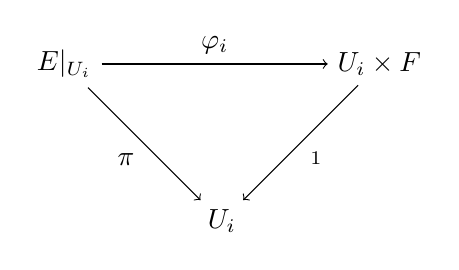
\begin{tikzpicture}
                \node (E) at (-2, 0) {$E|_{U_i}$};
                \node (UF) at (2, 0) {$U_i\times F$};
                \node (U) at (0, -2) {$U_i$};
                \draw[->] (E) -- node[above]{$\varphi_i$} (UF);
                \draw[->] (E) -- node[below left]{$\pi$} (U);
                \draw[->] (UF) -- node[below right]{$\pr_1$} (U);
            \end{tikzpicture}
        \end{gather*}
        It should be noted that the existence of such a cover is not a trivial matter. The general definition becomes quite involved when allowing for arbitrary smooth 2-spaces $B$. For convenience, it will always be assumed that $B$ is an ordinary smooth space regarded as a 2-space with only trivial morphisms.

        As was the case in \cref{bundle:fibre_bundle}, one can also characterize locally trivial 2-bundles by their transition data. Since the trivilizations $\varphi_i$ are equivalences, they admit an inverse (up to an invertible 2-map) and one can thus construct transition maps $\varphi_i\circ\varphi_j^{-1}=U_{ij}\times F\cong U_{ij}\times F$ as usual. By the commutative diagram above, these transition maps only act on the fibre $F$. Because $\varphi_i\circ\varphi_j^{-1}$ is itself an (auto)equivalence, the action on $F$ is given by a functor $g_{ij}:U_{ij}\rightarrow\mathbf{Aut}(F)$, where the 2-space $\mathbf{Aut}(F)$ is the (coherent) automorphism 2-group of $F$.

        The interesting (and important) part is how the cocycle conditions (\cref{bundle:G_cocycle_condition} and \cref{bundle:G_cocycle_conditions}) for the maps $g_{ij}$ are modified. Since the equivalences $g_{ij}$ are only invertible up to 2-morphisms, one cannot expect these conditions to hold as equations. Instead, two higher transition maps (i.e.~natural isomorphisms) $h_{ijk}:g_{ij}\circ g_{jk}\Rightarrow g_{ik}$ and $k_i:g_{ii}\Rightarrow\text{id}_F$ are obtained. These higher data should in turn satisfy the necessary conditions coming from associativity and unitality constraints (similar to the coherence conditions from \cref{section:hda_group_cohomology}).
    }

    \newdef{$G$-bundle}{\index{principal!bundle}
        A locally trivial 2-bundle with typical fibre $F$ is said to have the 2-group $G$ as its structure (2-)group if the transition data factor through an action $G\rightarrow\mathbf{Aut}(F)$. If $F=G$, the 2-bundle is called a \textbf{principal $G$-2-bundle}.
    }
    \begin{remark}[Gerbes]\index{gerbe}
        If the transition maps $k_i$ are chosen to be trivial and $G$ is chosen to be, respectively, the trivial Lie 2-group associated to an Abelian Lie group $G$ or the automorphism 2-group of a Lie group $H$, one obtains Abelian and non-Abelian \textit{gerbes}. In fact, it can be shown that the 2-category of principal $2$-bundles is equivalent to the 2-category of gerbes for every Lie 2-group of the aforementioned type.
    \end{remark}

    By categorifying \cref{bundle:holonomy_functor} of principal connections, one can define connections for principal $n$-bundles.
    \newdef{$n$-connection}{\index{connection!principal}
        Let $M$ be a smooth space and let $G$ be a Lie $n$-groupoid. Given a locally trivial principal $n$-bundle $P$ over $M$, an $n$-connection with $n$-holonomy is defined by the following data:
        \begin{itemize}
            \item for every coordinate chart $U_i\subseteq M$ a local holonomy $n$-functor
            \begin{gather}
                \mathrm{hol}_i:\mathcal{P}_n(U_i)\rightarrow G\,,
            \end{gather}
            \item for every double intersection $U_{ij}$ a 1-transfor (\cref{cat:transfor})
            \begin{gather}
                g_{ij}:\mathrm{hol}_i\Rightarrow\mathrm{hol}_j\,,
            \end{gather}
            \item for every triple intersection $U_{ijk}$ a 2-transfor
            \begin{gather}
                f_{ijk}:g_{ij}\circ g_{jk}\Rrightarrow g_{ik}\,,
            \end{gather}
            \item and so on ...
        \end{itemize}
        This is equivalently given by a global $n$-functor
        \begin{gather}
            \mathrm{hol}:\mathcal{P}_n(M)\rightarrow\mathbf{Trans}_n(P)\,.
        \end{gather}
    }

    \todo{ADD GERBES (e.g.~BRYLINSKI)}

\section{Space and quantity}\label{section:space_and_quantity}

    In this section, the general notions of spaces and observables are reconsidered. From the start, everything will be formulated in an enriched setting, where $\mathcal{V}$ is a cosmos (\cref{cat:cosmos}). The categories of interest will also be assumed to be small.

    In \cref{section:smooth_spaces}, spaces modelled on a base space or, more generally, on a category of spaces were presented as (concrete) sheaves on a suitable site. Here, this notion is relaxed as much as possible.
    \newdef{Space}{\index{space}
        A (generalized) space modelled on a category $\mathbf{C}$ is a presheaf on $\mathbf{C}$.

        As before, the object $X(C)$ can be interpreted as the collection of `probes' from $C$ to $X$. The Yoneda lemma assures that ordinary test spaces in $\mathbf{C}$ can be viewed as spaces modelled on $\mathbf{C}$ and that their probes are indeed the ordinary maps in $\mathbf{C}$.
    }

    In a similar vein, one can define observables as maps out of a space.
    \newdef{Quantity}{\index{quantity}
        A (generalized\footnote{It is generalized because it `measures' a category instead of a single object.}) quantity on a category $\mathbf{C}$ is a copresheaf on $\mathbf{C}$.
    }

    \begin{property}[Isbell duality]\index{Isbell duality}
        Given a space $X$, one can look at the quantities that live on it (in ordinary geometry this would have been its algebra of functions). This defines a functor:
        \begin{gather}
            \mathcal{O}:\mathbf{Psh(C)}\rightarrow\mathbf{coPsh}^{\text{op}}(\mathbf{C}):X\mapsto\hom_{\mathbf{Psh(C)}}(X,\mathcal{Y}-)\,.
        \end{gather}
        Similarly, given a quantity $Q$ one can ask on which space it behaves as the algebra of functions. This also defines as functor:
        \begin{gather}
            \mathrm{Spec}:\mathbf{coPsh}^{\text{op}}(\mathbf{C})\rightarrow\mathbf{Psh(C)}:Q\mapsto\hom_{\mathbf{coPsh(C)}}(\mathcal{Y}^{\text{op}}-,Q)\,,
        \end{gather}
        where $\mathcal{Y}^{\text{op}}$ denotes the co-Yoneda embedding $\mathbf{C}\rightarrow\funccat{C}{\mathcal{V}}^{\text{op}}:c\mapsto\mathbf{C}(c,-)$.

        The incredible result is now that $(\mathcal{O}\dashv\mathrm{Spec})$ is an adjunction, called the \textbf{Isbell adjunction}. Objects that are preserved (up to isomorphism) under the associated (co)monad are said to be \textbf{Isbell selfdual}.
    \end{property}

    \begin{example}[Cartesian spaces]
        When working over the site $\mathbf{CartSp}$ (with its usual topology) and restricting to coherent sheaves and product-preserving presheaves, the Isbell adjunction maps spaces to smooth algebras.
    \end{example}